En este capítulo se presentan los conceptos matemáticos necesarios para comprender el funcionamiento de los sistemas de SLAM. Estos conceptos son fundamentales para entender cómo se representan matemáticamente los problemas de optimización en SLAM, desde la representación de poses y transformaciones, hasta la aplicación de métodos de optimización no lineal en espacios curvos. Además, se introducen métodos de image retrieval y de estimación de pose robusta.

\section{Modelos de cámara}

Una cámara proyecta el mundo 3D sobre una imagen 2D. Comprender cómo funciona este mapeo es fundamental para cualquier sistema basado en visión. A continuación se presenta el modelo pinhole, la abstracción más simple para cámaras de perspectiva, aunque existen modelos más complejos para lentes con mayor distorsión~\cite{usenko2018doublesphere}.

En el modelo de cámara pinhole, la cámara es un único punto en el espacio, el centro óptico, a través del cual pasan todos los rayos de luz. Un punto 3D $\mathbf{P}^c = [x, y, z]^T$, expresado en el sistema de referencia de la cámara, se proyecta como la intersección del rayo que lo une con el centro óptico y el plano de imagen, ubicado a una distancia focal $f$ (véase la Figura~\ref{fig:pinhole-model}). La función de proyección $\pi(\cdot)$, que mapea un punto 3D a coordenadas de píxel, se define como:
\begin{equation}
    \pi\!\left(\mathbf{P}^c\right) = \mathbf{u} =
    \begin{bmatrix}
        f_u \dfrac{x}{z} + c_x \\[6pt]
        f_v \dfrac{y}{z} + c_y
    \end{bmatrix},
    \label{eq:pinhole}
\end{equation}
donde $f_u$ y $f_v$ son las distancias focales en píxeles y $(c_x, c_y)$ es el punto principal, es decir, las coordenadas del eje óptico en el plano de imagen. Estos cuatro valores se denominan \textit{parámetros intrínsecos} de la cámara, y se agrupan en la matriz intrínseca $\mathbf{K}$:
\begin{equation}
    \mathbf{K} =
    \begin{bmatrix}
        f_u & 0   & c_x \\
        0   & f_v & c_y \\
        0   & 0   & 1
    \end{bmatrix}.
    \label{eq:intrinsics}
\end{equation}
Cuando el punto está expresado en un sistema de referencia global en lugar del sistema de la cámara, debe transformarse primero usando los \textit{parámetros extrínsecos}: una rotación $\mathbf{R}$ y una traslación $\mathbf{t}$ que describen la pose de la cámara en el mundo. La proyección completa es entonces
\begin{equation}
    \mathbf{u} = \pi\!\left(\mathbf{R}\,\mathbf{P}^w + \mathbf{t}\right).
    \label{eq:full_projection}
\end{equation}

\begin{figure}[ht]
    \centering
    \begin{subfigure}[b]{0.48\textwidth}
        \centering
        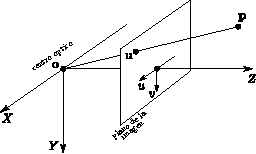
\includegraphics[width=\textwidth]{img/prev_concepts/pinhole-model-3d.pdf}
        \caption{Vista 3D: el punto $\mathbf{p}$ se proyecta a través del centro óptico sobre el plano de imagen, obteniéndose la observación $\mathbf{u}$.}
        \label{fig:pinhole-model-1}
    \end{subfigure}
    \hfill
    \begin{subfigure}[b]{0.48\textwidth}
        \centering
        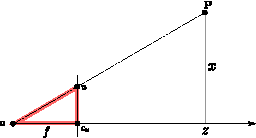
\includegraphics[width=\textwidth]{img/prev_concepts/pinhole-model-side-view.pdf}
        \caption{Vista lateral: se aprecia la distancia focal $f$ entre el centro óptico y el plano de imagen.}
        \label{fig:pinhole-model-2}
    \end{subfigure}
    \caption{Modelo de cámara pinhole.}
    \label{fig:pinhole-model}
\end{figure}

El proceso inverso, denominado desproyección (\textit{unprojection}), recupera un rayo en el espacio 3D a partir de una observación en píxeles. Dado que la profundidad se pierde durante la proyección, un único píxel corresponde a un rayo completo y no a un punto 3D único. Este rayo se representa como un vector de dirección unitario (\textit{bearing vector}):
\begin{equation}
    \mathbf{b} = \pi^{-1}(\mathbf{u}) =
    \frac{1}{\sqrt{m_x^2 + m_y^2 + 1}}
    \begin{bmatrix} m_x \\ m_y \\ 1 \end{bmatrix},
    \quad
    m_x = \frac{u - c_x}{f_u}, \quad m_y = \frac{v - c_y}{f_v}.
    \label{eq:unprojection}
\end{equation}

En la práctica, las lentes reales introducen distorsión que hace que la imagen se desvíe del modelo pinhole ideal. Existen modelos de cámara más complejos que incorporan parámetros adicionales para caracterizar estos efectos, como la distorsión radial, que hace que las líneas rectas aparezcan curvadas. Durante la \textit{calibración de la cámara} se optimizan estos parámetros, tras lo cual los puntos 3D pueden proyectarse, y los puntos 2D desproyectarse de acuerdo a las ecuaciones del modelo con los parámetros establecidos.

\section{Grafo de factores}

Un grafo de factores es un grafo que representa la factorización de una función. Es decir, un
grafo de factores representa una función $g()$ que se puede descomponer mediante el producto de
funciones $f_i()$ que dependen de un subconjunto de las variables de $g$, esto es:
\[
g(X_1, \ldots, X_n) = \prod_{i} f_i(S_i) \quad \text{con } S_i \subseteq \{X_1, \ldots, X_n\}.
\]
Se compone de dos elementos principales:
\begin{itemize}
    \item \textbf{Nodos:} Representan las variables $X_i$ de la función $g()$.
    \item \textbf{Factores:} Representan las restricciones o relaciones entre los nodos. Cada función $f_i(S_i)$
    se denomina un factor y modela cómo interactúan las variables en $S_i$. Estos factores
    introducen las relaciones entre las variables que se deben cumplir para obtener una solución
    coherente al problema de estimación.
\end{itemize}

A continuación se presenta un ejemplo de un grafo de factores que representa la función
$g()$. En este caso, los nodos $X_1, X_2, X_3, X_4$ representan las variables, y los factores
$f_1, f_2, f_3$ representan las restricciones que vinculan estas variables:
\[
g(X_1, X_2, X_3, X_4) = f_1(X_1, X_2, X_4)\,f_2(X_2, X_3)\,f_3(X_3).
\]

\begin{figure}[h]
    \centering
    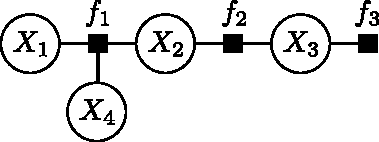
\includegraphics[width=0.4\linewidth]{img/prev_concepts/factor-graph.pdf}
    \caption{Ejemplo de un grafo de factores que representa la función $g()$.}
    \label{fig:factor_graph}
\end{figure}

En sistemas VIO y VI-SLAM, los grafos de factores se utilizan para modelar las relaciones
entre las variables de estado del sistema. Estas variables incluyen la posición y orientación del
dispositivo en diferentes instantes de tiempo (conocidas como poses) y la posición de puntos clave
(landmarks) en el espacio 3D. En este contexto, los nodos representan las poses del dispositivo
y las posiciones de los landmarks en el espacio. Los factores, por otro lado, representan las
restricciones basadas en las observaciones realizadas por los sensores del sistema, como cámaras
o IMUs. Estos factores modelan las relaciones entre diferentes poses o entre poses y landmarks,
basándose en las mediciones obtenidas. El propósito de utilizar un grafo de factores en SLAM es
encontrar las estimaciones de las variables que mejor satisfagan todas las restricciones impuestas
por las mediciones sensoriales. Este proceso se realiza mediante algoritmos de optimización no
lineal, como Gauss-Newton o Levenberg-Marquardt. En la Figura \ref{fig:real_factor_graph}, se muestra un ejemplo de
un grafo de factores de un sistema SLAM.

\begin{figure}[h]
    \centering
    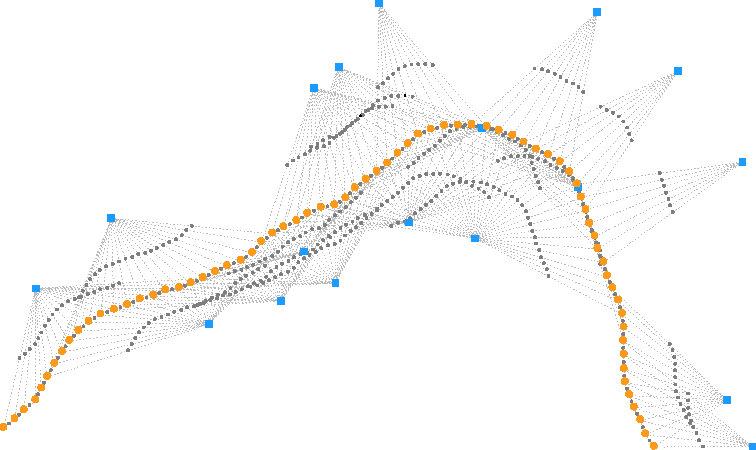
\includegraphics[width=0.4\linewidth]{img/prev_concepts/real-factor-graph.pdf}
    \caption{Ejemplo de un grafo de factores de un sistema SLAM.}
    \label{fig:real_factor_graph}
\end{figure}

\subsection{Error de reproyección}

El error de reproyección mide la distancia entre la posición observada de un punto en la
imagen de una cámara y la posición proyectada de ese mismo punto, calculada a partir de su
posición estimada en el espacio 3D y la pose de la cámara. Este error se mide típicamente en
píxeles y se puede expresar como:
\[
e_{\text{reproyección}} = \|\mathbf{p}_j - \hat{\mathbf{p}}_j\|,
\]
donde:
\begin{itemize}
    \item $\mathbf{p}_j \in \mathbb{R}^2$ son las coordenadas observadas del punto $j$ en la imagen,
    \item $\hat{\mathbf{p}}_j \in \mathbb{R}^2$ son las coordenadas proyectadas del punto $j$ en la imagen, calculadas a partir de su posición estimada en 3D y la pose de la cámara.
\end{itemize}

\[
\hat{\mathbf{u}}
=
\pi(\mathbf{T}_{cw}\mathbf{p}_w),
\]

\begin{figure}[h]
    \centering
    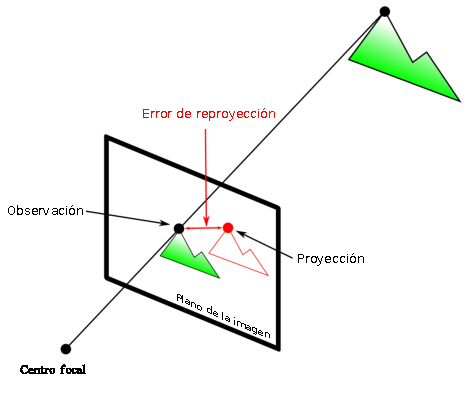
\includegraphics[width=0.4\linewidth]{img/prev_concepts/reproj-error.pdf}
    \caption{Ejemplo de un error de reproyección en un sistema SLAM.}
    \label{fig:reproj_error}
\end{figure}

En sistemas SLAM, el error de reproyección se utiliza para ajustar la estimación tanto de
la trayectoria del dispositivo como de la posición de los puntos clave en el entorno. El objetivo
es minimizar la suma de los errores de reproyección para todas las observaciones y cámaras, lo
cual se expresa mediante la siguiente función de costo:
\[
\min \sum_{i} \sum_{j} \|\mathbf{p}_{i,j} - \hat{\mathbf{p}}_{i,j}\|^2,
\]
donde:
\begin{itemize}
    \item $\mathbf{p}_{i,j} \in \mathbb{R}^2$ son las coordenadas observadas del punto $j$ en la imagen de la cámara $i$,
    \item $\hat{\mathbf{p}}_{i,j} \in \mathbb{R}^2$ son las coordenadas proyectadas del punto $j$ en la imagen de la cámara $i$, calculadas a partir de la estimación de su posición 3D y la pose de la cámara.
\end{itemize}

Este proceso de optimización ajusta tanto las posiciones estimadas de los puntos clave en
3D como las poses de las cámaras, reduciendo la discrepancia entre las proyecciones estimadas
y las observaciones reales, mejorando así la precisión en la localización del dispositivo y la
reconstrucción del mapa. En la Figura \ref{fig:reproj_error} se muestra una representación gráfica del error de
reproyección.

\subsection{Error de pose relativa}

El error de pose relativa mide la discrepancia entre la transformación relativa estimada entre
dos poses consecutivas y la transformación relativa observada por los sensores. Se utiliza en la
optimización de grafos de poses para corregir la trayectoria estimada del dispositivo.

%Se adopta la notación $\mathbf{T}_{ij} \in SE(3)$ para referirse a la transformación que lleva
%puntos expresados en el frame $j$ al frame $i$, es decir, la pose del frame $j$ vista desde el
%frame $i$. En particular, $\mathbf{T}_{wi}$ denota la pose del frame $i$ en coordenadas del
%mundo. La transformación relativa entre dos frames se obtiene entonces como:
La transformación relativa entre dos poses consecutivas de cámaras $i$ y $j$ se obtiene como:
\[
\mathbf{T}_{ij} = \mathbf{T}_{wi}^{-1}\,\mathbf{T}_{wj}.
\]

Dadas las poses estimadas $\hat{\mathbf{T}}_{wi}$ y $\hat{\mathbf{T}}_{wj}$, y una medición de la transformación relativa $\tilde{\mathbf{T}}_{ij}$ provista por los sensores, el error de pose relativa se define como:
\[
\mathbf{e}_{ij}
= \log\!\left(\tilde{\mathbf{T}}_{ij}^{-1}\,\hat{\mathbf{T}}_{wi}^{-1}\,\hat{\mathbf{T}}_{wj}\right)^\vee
\in \mathbb{R}^6.
\]

El término $\hat{\mathbf{T}}_{wi}^{-1}\hat{\mathbf{T}}_{wj} = \hat{\mathbf{T}}_{ij}$ es la transformación relativa estimada. El factor $\tilde{\mathbf{T}}_{ij}^{-1}\hat{\mathbf{T}}_{ij}$ compara medición y estimación. Cuando ambas coinciden el resultado es la identidad y el error es nulo. Dado que el resultado de dicha comparación pertenece a $SE(3)$ y el error debe expresarse en $\mathbb{R}^6$ para poder optimizarse, se aplica el mapa logarítmico de la pose seguido del operador $(\cdot)^\vee$, que extrae el vector de coordenadas. Estos conceptos, junto con la estructura de $SE(3)$, se introducen en la Sección~\ref{sec:lie}.

El objetivo de la optimización es minimizar la suma de los errores para todas las restricciones del grafo:
\[
\min \sum_{(i,j)} \left\|\log\!\left(\tilde{\mathbf{T}}_{ij}^{-1}\hat{\mathbf{T}}_{ij}\right)^\vee\right\|^2.
\]

Este tipo de error se utiliza, por ejemplo, al incorporar restricciones de ciclos en sistemas SLAM, donde una detección de ciclo introduce una nueva restricción entre poses no consecutivas del grafo.

% TODO: agregar figura de un pose graph con loop constraints?

\section{Minimos cuadrados}

El problema de mínimos cuadrados es una técnica fundamental en estadística y optimización matemática que se utiliza para ajustar un modelo a un conjunto de datos observados. Su objetivo es encontrar la mejor aproximación posible de los parámetros de un modelo, de manera que se minimice la diferencia entre las predicciones del modelo y los datos observados. El enfoque de mínimos cuadrados busca minimizar el error total o residual, que es la suma de los cuadrados de las diferencias entre los valores observados y los valores estimados por el modelo. Matemáticamente, el problema puede expresarse como:
\[
\min_{\mathbf{x}} \sum_{i=1}^{n} \bigl(y_i - f(x_i, \mathbf{x})\bigr)^2,
\]
donde:
\begin{itemize}
    \item $x_i$ son las entradas conocidas (las variables independientes),
    \item $y_i$ son los valores observados (las variables dependientes),
    \item $\mathbf{x}$ es el vector de parámetros del modelo a estimar,
    \item $f(x_i, \mathbf{x})$ es el modelo que se ajusta a los datos observados.
\end{itemize}

El problema de mínimos cuadrados no lineales extiende el enfoque de mínimos cuadrados al caso en el que el modelo $f(x_i)$ no es una función lineal. A diferencia del caso lineal, donde la solución se obtiene directamente resolviendo un sistema de ecuaciones, en el caso no lineal no existe una solución analítica directa. La resolución se basa en métodos iterativos que ajustan los parámetros del modelo calculando gradientes, Jacobianos y Hessianos en cada iteración.

\paragraph{Gradiente}

El gradiente de una función escalar $F(\mathbf{x})$ es un vector de derivadas parciales:
\[
\nabla F(\mathbf{x}) =
\begin{bmatrix}
\dfrac{\partial F}{\partial x_1} &
\dfrac{\partial F}{\partial x_2} &
\cdots &
\dfrac{\partial F}{\partial x_n}
\end{bmatrix}^\top.
\]
Indica la dirección de mayor aumento de $F$ y se utiliza para determinar en qué dirección ajustar los parámetros para reducir la función de costo.

\paragraph{Jacobiano}

La matriz Jacobiana de una función vectorial $\mathbf{f}(\mathbf{x})$ contiene las derivadas parciales de cada componente de $\mathbf{f}$ respecto a cada componente de $\mathbf{x}$:
\[
\mathbf{J}(\mathbf{x}) =
\begin{bmatrix}
\dfrac{\partial f_1}{\partial x_1} & \dfrac{\partial f_1}{\partial x_2} & \cdots & \dfrac{\partial f_1}{\partial x_n} \\[8pt]
\dfrac{\partial f_2}{\partial x_1} & \dfrac{\partial f_2}{\partial x_2} & \cdots & \dfrac{\partial f_2}{\partial x_n} \\[8pt]
\vdots & \vdots & \ddots & \vdots \\[4pt]
\dfrac{\partial f_m}{\partial x_1} & \dfrac{\partial f_m}{\partial x_2} & \cdots & \dfrac{\partial f_m}{\partial x_n}
\end{bmatrix}.
\]
Proporciona una aproximación lineal de $\mathbf{f}$ alrededor de un punto dado y es crucial en métodos iterativos de optimización.

\paragraph{Hessiano}

La matriz Hessiana de una función escalar $F(\mathbf{x})$ contiene las segundas derivadas parciales de $F$:
\[
\mathbf{H}(\mathbf{x}) =
\begin{bmatrix}
\dfrac{\partial^2 F}{\partial x_1^2} & \dfrac{\partial^2 F}{\partial x_1 \partial x_2} & \cdots & \dfrac{\partial^2 F}{\partial x_1 \partial x_n} \\[8pt]
\dfrac{\partial^2 F}{\partial x_2 \partial x_1} & \dfrac{\partial^2 F}{\partial x_2^2} & \cdots & \dfrac{\partial^2 F}{\partial x_2 \partial x_n} \\[8pt]
\vdots & \vdots & \ddots & \vdots \\[4pt]
\dfrac{\partial^2 F}{\partial x_n \partial x_1} & \dfrac{\partial^2 F}{\partial x_n \partial x_2} & \cdots & \dfrac{\partial^2 F}{\partial x_n^2}
\end{bmatrix}.
\]
Es utilizada en métodos de optimización de segundo orden para capturar la curvatura de la función de costo y proporcionar información más precisa sobre la topología local de $F(\mathbf{x})$.

El método de Gauss-Newton es un algoritmo iterativo utilizado para resolver problemas de mínimos cuadrados no lineales. Se basa en una aproximación lineal de la función objetivo, lo que permite transformar el problema no lineal en una secuencia de problemas de mínimos cuadrados lineales. Es particularmente eficiente cuando el modelo no se desvía significativamente de un comportamiento lineal, evitando el cálculo completo de la matriz Hessiana.

Dado el problema de mínimos cuadrados no lineales:
\[
\min_{\mathbf{x}} \sum_{i=1}^{n} \bigl(y_i - f(x_i, \mathbf{x})\bigr)^2,
\]
el método aproxima $f(x_i, \mathbf{x})$ mediante una expansión de Taylor de primer orden entorno a la estimación actual $\mathbf{x}_k$:
\[
f(x_i, \mathbf{x}) \approx f(x_i, \mathbf{x}_k) + \mathbf{J}(x_i)(\mathbf{x} - \mathbf{x}_k),
\]
donde $\mathbf{J}(x_i)$ es la matriz Jacobiana de $f$ respecto a $\mathbf{x}$, evaluada en $\mathbf{x}_k$. Sustituyendo en la función objetivo se obtiene un problema de mínimos cuadrados lineal. Igualando su gradiente a cero se llega al sistema de ecuaciones normales:
\[
\mathbf{J}^\top \mathbf{J}\,\Delta\mathbf{x} = \mathbf{J}^\top \mathbf{r},
\]
donde $\mathbf{r} = y_i - f(x_i, \mathbf{x}_k)$ son los residuales y $\Delta\mathbf{x}$ es el incremento de los parámetros. Luego los parámetros se actualizan como:
\[
\mathbf{x}_{k+1} = \mathbf{x}_k + \Delta\mathbf{x}.
\]

Este proceso se repite hasta que $\|\Delta\mathbf{x}\|$ es suficientemente pequeño, indicando convergencia. El método es computacionalmente eficiente porque aproxima la Hessiana mediante $\mathbf{J}^\top\mathbf{J}$. Sin embargo, puede fallar cuando la aproximación lineal no es suficiente. En esos casos se puede utilizar el método de Levenberg-Marquardt, que introduce un término de amortiguamiento (\textit{damping factor}) para estabilizar la convergencia~\cite{nocedal2006numerical}.

\section{Manifolds, Lie Groups, and Optimization on $SE(3)$}
\label{sec:lie}

% https://ethaneade.com/lie.pdf
% https://asrl.utias.utoronto.ca/~tdb/bib/barfoot_ser17.pdf

\subsection{Manifolds}

Many quantities in robotics and computer vision cannot be represented properly using unconstrained
Euclidean vectors. Rotations are a classical example: a rotation matrix must satisfy orthogonality
constraints and therefore cannot vary freely in $\mathbb{R}^{3\times3}$.

To describe these constrained spaces, the concept of a manifold is introduced.

A manifold is a space that may have a curved global structure, but locally resembles Euclidean
space. This means that, around every point, it is possible to define a local coordinate system
where standard vector operations are valid.

Optimization methods such as Gauss-Newton rely on local linear approximations. Therefore, when
optimizing quantities defined on manifolds, updates are performed in a local Euclidean
approximation called the tangent space.

For pose estimation problems, camera poses lie on the manifold $SE(3)$.

\subsection{Lie Groups}

A Lie group is a mathematical structure that combines:

\begin{enumerate}
\item a smooth manifold structure,
\item and a group structure.
\end{enumerate}

The manifold structure enables local differential operations such as derivatives and linearization, while the group structure defines valid composition and inversion operations.

The term \textbf{Lie} indicates that the group operations are smooth and differentiable, which allows optimization and calculus to be performed on the manifold.

\subsection{The Special Orthogonal Group (SO(3))}

Rotations in 3D space belong to the Special Orthogonal group:

\[
SO(3) = \left\{ \mathbf{R} \in \mathbb{R}^{3\times3} \mid \mathbf{R}^\top \mathbf{R} = \mathbf{I},\ \det(\mathbf{R}) = 1 \right\}
\]

The properties of a rotation matrix are:

\begin{itemize}
    \item orthogonality:
    \[
    \mathbf{R}^{-1} = \mathbf{R}^\top,
    \]

    \item determinant equal to 1,

    \item preservation of distances and angles.
\end{itemize}

Since a rotation matrix has nine elements but only three degrees of freedom, rotations form a constrained manifold rather than a Euclidean vector space.

\subsection{The Special Euclidean Group $(SE(3))$}

Rigid body transformations in 3D belong to the Special Euclidean group:

\[
SE(3) = \left\{ \mathbf{T} = \begin{bmatrix} \mathbf{R} & \mathbf{t} \\ \mathbf{0}^\top & 1 \end{bmatrix} \,|\, \mathbf{R}\in SO(3),\ \mathbf{t}\in\mathbb{R}^3 \right\}
\]

A transformation acts on a 3D point as

$$
\mathbf{p}' = \mathbf{R}\mathbf{p}+\mathbf{t}.
$$

Using homogeneous coordinates:

$$
\tilde{\mathbf{p}}' =
\mathbf{T}\tilde{\mathbf{p}}.
$$

The group operation corresponds to transformation composition:

$$
\mathbf{T}_{ac}
=
\mathbf{T}_{ab}\mathbf{T}_{bc}.
$$

The inverse transformation is

$$
\mathbf{T}^{-1} =
\begin{bmatrix}
\mathbf{R}^\top & -\mathbf{R}^\top\mathbf{t}\\
\mathbf{0}^\top & 1
\end{bmatrix}.
$$

The space $SE(3)$ has six degrees of freedom: three rotational and three translational.

\subsection{Tangent Spaces and Lie Algebras}

Optimization algorithms require additive updates:

$$
\mathbf{x}
\leftarrow
\mathbf{x}+\Delta\mathbf{x}.
$$

However, poses in $SE(3)$ cannot be updated directly using vector addition because $SE(3)$ is not a vector space.

Instead, updates are computed in the tangent space of the manifold.

The tangent space associated with a Lie group is called its Lie algebra.

For $SE(3)$, the Lie algebra is denoted by

\[
\mathfrak{se}(3).
\]

Unlike $SE(3)$, the Lie algebra is a vector space, meaning: vectors can be added, scaled and optimized using standard linear algebra techniques.

An element of $\mathfrak{se}(3)$ is represented as

\[
\boldsymbol{\xi}=
\begin{bmatrix}
\boldsymbol{\rho}\\
\boldsymbol{\phi}
\end{bmatrix}
\in\mathbb{R}^6,
\]

where:

\begin{itemize}
    \item $\boldsymbol{\rho}\in\mathbb{R}^3$ represents translation,
    \item $\boldsymbol{\phi}\in\mathbb{R}^3$ represents rotation.
\end{itemize}

The Lie algebra provides a minimal local parameterization of rigid body motions.

\subsection{The Hat Operator}

The hat operator $(\cdot)^\wedge$ maps a vector $\boldsymbol{\xi}\in\mathbb{R}^6$ to
its matrix representation in the Lie algebra, and its inverse, the vee operator
$(\cdot)^\vee$, maps back to vector form. This correspondence is used by the exponential
map to move between the algebra and the group.

\subsection{The Exponential Map and Log Map}

The exponential map and the logarithmic map are the two operations that connect the Lie algebra
with the Lie group:

\[
\exp: \mathfrak{se}(3) \rightarrow SE(3), \qquad \log: SE(3) \rightarrow \mathfrak{se}(3).
\]

The exponential map converts a tangent vector $\boldsymbol{\xi}^{\wedge}$ into a valid rigid
body transformation:

\[
\mathbf{T} = \exp(\boldsymbol{\xi}^{\wedge}),
\]

guaranteeing that optimized poses remain on the manifold. The logarithmic map is its
inverse: given a transformation $\mathbf{T}\in SE(3)$, it recovers the corresponding Lie
algebra element,

\[
\boldsymbol{\xi}^{\wedge} = \log(\mathbf{T}).
\]

Together, these maps allow moving freely between the curved manifold and the flat tangent
space where standard linear operations are valid.

\begin{figure}[h]
    \centering
    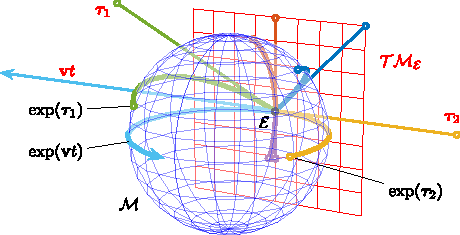
\includegraphics[width=0.4\linewidth]{img/prev_concepts/lie-algebra.pdf}
    \caption{Representación visual de un grupo de Lie, su álgebra de Lie asociada, y
    los mapas exponencial y logarítmico que conectan ambos espacios.}
    \label{fig:lie_algebra}
\end{figure}

\subsection{Pose Updates in Optimization}

Suppose a pose estimate $\mathbf{T}$ must be refined by a small increment $\Delta\boldsymbol{\xi}$.

Instead of using an invalid additive update:

\[
\mathbf{T}
\leftarrow
\mathbf{T}
+
\Delta\mathbf{T},
\]

the update is performed on the manifold:

\[
\mathbf{T}
\leftarrow
\exp(\Delta\boldsymbol{\xi}^{\wedge})
\mathbf{T}.
\]

This is called a left perturbation model.

The increment is computed in Euclidean space, mapped to the manifold using the exponential
map, and composed with the current estimate.

This framework enables standard nonlinear least-squares optimization while respecting the
geometry of rigid body transformations.

\subsection{Representación Adjunta de \texorpdfstring{$SE(3)$}{SE(3)}}
% TODO: rever escritura de esto. por ejemplo: twist -> perturbación. pero el concepto y las referencias están.

La representación adjunta es un mapa lineal asociado a cada elemento del
grupo de Lie que describe cómo actúa el grupo sobre su álgebra de Lie por
conjugación. Para un elemento $T \in SE(3)$, el mapa adjunto
$\mathrm{Ad}_T : \mathfrak{se}(3) \to \mathfrak{se}(3)$ se define como
%
\begin{equation}
    \mathrm{Ad}_T(\xi) = T\,\xi\,T^{-1},
\end{equation}
%
donde $\xi \in \mathfrak{se}(3)$ es un elemento del álgebra de Lie. En su
representación matricial de $6\times6$, para $T = (R,\,p) \in SE(3)$, el
mapa adjunto toma la forma~\cite{Lynch2017}
%
\begin{equation}
    [\mathrm{Ad}_T] =
    \begin{bmatrix}
        R          & 0 \\
        [p]_\times R & R
    \end{bmatrix}
    \in \mathbb{R}^{6\times6},
\end{equation}
%
donde $[p]_\times$ denota la matriz antisimétrica asociada al vector de
traslación $p$.

Una propiedad fundamental de la representación adjunta, empleada
extensamente en robótica, es que permite cambiar el marco de referencia en
el que se expresa un twist. Dado un twist $\xi_b \in \mathbb{R}^6$ expresado
en el marco $\{b\}$, su expresión equivalente en el marco $\{a\}$ está dada
por~\cite{Lynch2017}
%
\begin{equation}
    \xi_a = [\mathrm{Ad}_{T_{ab}}]\,\xi_b,
    \label{eq:adjoint_twist}
\end{equation}
%
donde $T_{ab} \in SE(3)$ es la transformación homogénea que relaciona el
marco $\{b\}$ con el marco $\{a\}$. Esta identidad es consecuencia directa
de la relación
%
\begin{equation}
    T\exp(\xi)\,T^{-1} = \exp\!\bigl([\mathrm{Ad}_T]\,\xi\bigr),
\end{equation}
%
que vincula la acción adjunta con el mapa exponencial del
grupo~\cite{Lynch2017}.


% optimization happens in tangent spaces,
% while the actual states live on manifolds.

\section{Bundle Adjustment}

Bundle adjustment jointly estimates camera poses and 3D landmark positions by minimizing
reprojection errors across all observations.

Given a landmark $\mathbf{x}_l$, a camera pose $\mathbf{x}_p$, and an observed image
point $\mathbf{u}$, the predicted projection is
\[
\hat{\mathbf{u}}
=
\pi(\mathbf{x}_p, \mathbf{x}_l),
\]
where $\pi(\cdot)$ denotes the camera projection model. The reprojection residual is then
\[
\mathbf{r}
=
\mathbf{u}
-
\hat{\mathbf{u}}.
\]

The optimization variables are split into a pose component $\xi$, collecting all camera
poses, and a landmark component $x_l$, collecting all 3D point positions. Since camera
poses lie on the $SE(3)$ manifold, they are parameterized locally via perturbations in the
Lie algebra $\mathfrak{se}(3)$, while landmarks are represented directly in $\mathbb{R}^3$.

The bundle adjustment problem minimizes the sum of squared reprojection residuals over
all cameras $i$ and their observed landmarks $j \in O(i)$:
\[
E(\xi, x_l)
=
\sum_i \sum_{j \in O(i)}
\left\|
\mathbf{r}_{ij}(\xi, x_l)
\right\|^2.
\]

Linearizing each residual around the current estimate $x_0 = (\xi^0, x_l^0)$ gives
\[
\mathbf{r}(x)
\approx
\mathbf{r}(x_0)
+
\begin{pmatrix}
\mathbf{J}_{\xi} & \mathbf{J}_{l}
\end{pmatrix}
\begin{pmatrix}
\Delta \xi \\
\Delta x_l
\end{pmatrix},
\]

where
\[
\mathbf{J}_{\xi} = \frac{\partial \mathbf{r}}{\partial \xi} \Big|_{x_0}, \quad
\mathbf{J}_{l} = \frac{\partial \mathbf{r}}{\partial x_l} \Big|_{x_0}, \quad
\Delta x = x - x_0
\]

so the problem reduces at each iteration to
\[
\min_{\Delta \xi,\, \Delta x_l}
\left\|
\mathbf{r}(x_0)
+
\begin{pmatrix}
\mathbf{J}_{\xi} & \mathbf{J}_{l}
\end{pmatrix}
\begin{pmatrix}
\Delta \xi \\
\Delta x_l
\end{pmatrix}
\right\|^2.
\]


The optimal increments are found by solving the corresponding normal equations,
\[
\begin{pmatrix}
\mathbf{H}_{\xi\xi} & \mathbf{H}_{\xi l} \\
\mathbf{H}_{l\xi} & \mathbf{H}_{ll}
\end{pmatrix}
\begin{pmatrix}
-\Delta\boldsymbol{\xi} \\
-\Delta\mathbf{x}_l
\end{pmatrix}
=
\begin{pmatrix}
\mathbf{b}_\xi \\
\mathbf{b}_l
\end{pmatrix},
\]
where
\begin{align}
\mathbf{H}_{\xi\xi} &= \mathbf{J}_\xi^\top \mathbf{J}_\xi, &
\mathbf{H}_{ll} &= \mathbf{J}_l^\top \mathbf{J}_l, \\
\mathbf{H}_{\xi l} &= \mathbf{J}_\xi^\top \mathbf{J}_l = \mathbf{H}_{l\xi}^\top, \\
\mathbf{b}_\xi    &= \mathbf{J}_\xi^\top \mathbf{r},    &
\mathbf{b}_l    &= \mathbf{J}_l^\top \mathbf{r}.
\end{align}
The system matrix has size $(N_\xi + 3n_l)^2$, where $N_\xi$ is the total number of pose
parameters and $n_l$ is the number of landmarks. This can become impractically large
(millions of rows and columns) for typical map sizes. In the next sections, we will show
more efficient ways to solve this system by exploiting its structure.

Camera poses are then updated on the manifold via the exponential map,
\[
\mathbf{x}_p
\leftarrow
\exp(\Delta \boldsymbol{\xi}_i^\wedge)\,\mathbf{x}_p,
\],
while landmark positions are updated additively:
\[
\mathbf{x}_l
\leftarrow
\mathbf{x}_l + \Delta \mathbf{x}_l.
\]

\begin{figure}[h]
    \centering
    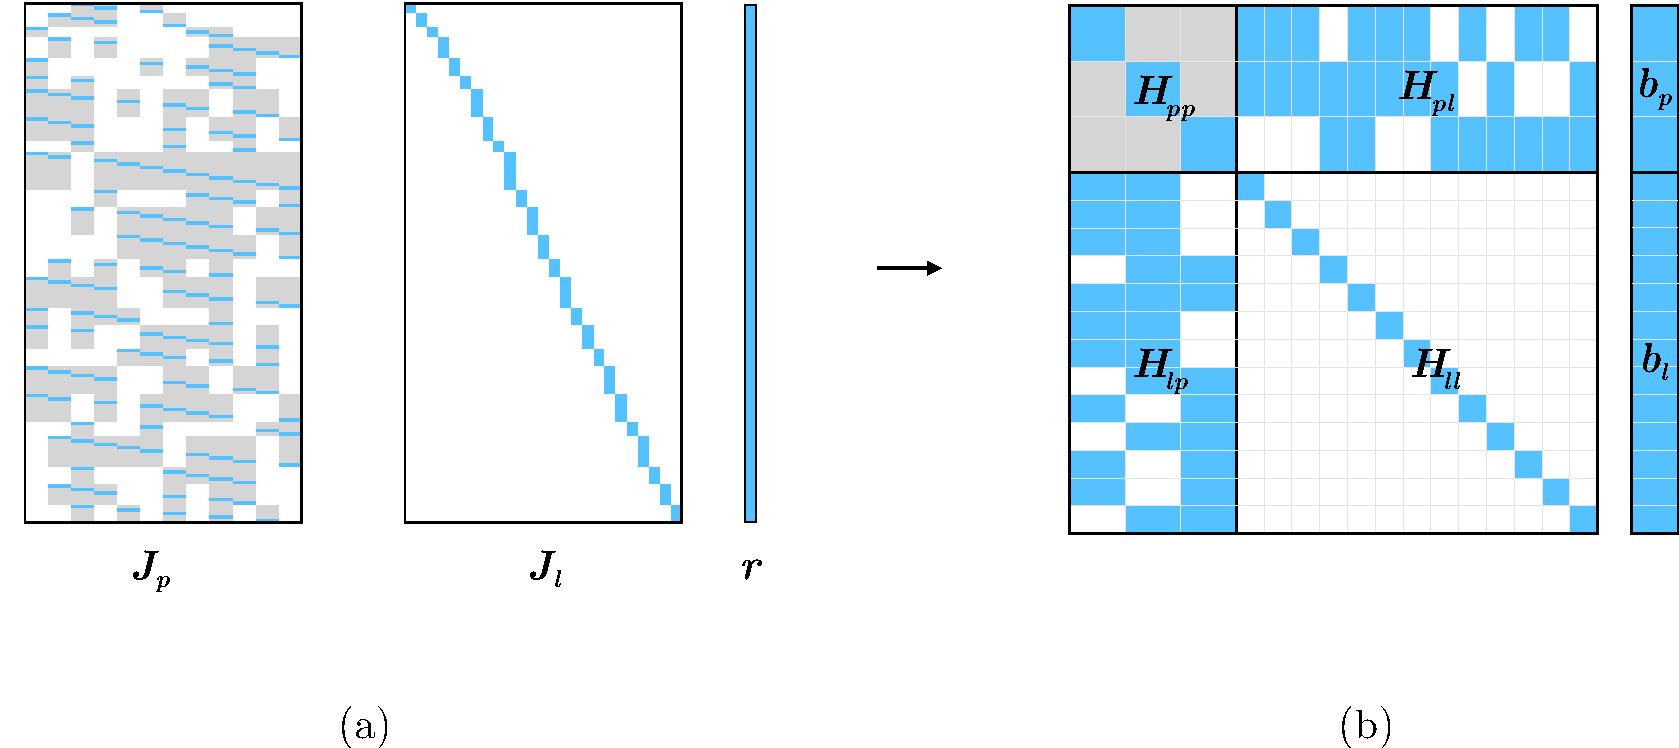
\includegraphics[width=0.7\linewidth]{img/prev_concepts/normal-equations.pdf}
    \caption{Ecuaciones normales y matriz Hessiana.}
    \label{fig:normal-equations}
\end{figure}

\subsection{Complemento de Schur}

A very common way to solve the normal equations is by applying the Schur complement trick.
Partitioning the system into pose variables $\Delta\mathbf{\xi}$ and landmark variables
$\Delta\mathbf{x}_l$, one forms the reduced camera system (RCS):
\[
\tilde{\mathbf{H}}_{\xi\xi}\,(-\Delta\mathbf{\xi}) = \tilde{\mathbf{b}}_\xi,
\]
with
\begin{align}
\tilde{\mathbf{H}}_{\xi\xi} &= \mathbf{H}_{\xi\xi} - \mathbf{H}_{\xi l}\mathbf{H}_{ll}^{-1}\mathbf{H}_{l\xi}, \\
\tilde{\mathbf{b}}_\xi    &= \mathbf{b}_\xi   - \mathbf{H}_{\xi l}\mathbf{H}_{ll}^{-1}\mathbf{b}_l.
\end{align}
The solution $\Delta\mathbf{\xi}^*$ of this system is identical to the pose component of the
full solution, but the system matrix now has size $N_\xi^2$, typically in the order of thousands
$\times$ thousands. Since $\mathbf{H}_{ll}$ is block-diagonal with $3\times3$ blocks, the
multiplication by $\mathbf{H}_{ll}^{-1}$ is cheap. Given the optimal pose update
$\Delta\mathbf{\xi}^*$, the optimal landmark update is recovered by back-substitution:
\[
\Delta\mathbf{x}_l^* = -\mathbf{H}_{ll}^{-1}\bigl(\mathbf{b}_l - \mathbf{H}_{l\xi}\,(-\Delta\mathbf{\xi}^*)\bigr).
\]

\subsection{Factorización QR}

An alternative to the Schur complement is to apply a QR decomposition directly to the
landmark Jacobian. Decomposing $\mathbf{J}_l = \mathbf{Q}\mathbf{R}$, where $\mathbf{Q}$
is orthogonal and $\mathbf{R}$ is upper-triangular, and partitioning $\mathbf{Q} =
[\mathbf{Q}_1\ \mathbf{Q}_2]$ conformally with the nonzero rows of $\mathbf{R}$, the
$\ell_2$-norm is invariant under orthogonal transformations, so the objective becomes
\begin{align}
\left\|
\mathbf{r}
+
\begin{pmatrix} \mathbf{J}_{\xi} & \mathbf{J}_l \end{pmatrix}
\begin{pmatrix} \Delta\boldsymbol{\xi} \\ \Delta\mathbf{x}_l \end{pmatrix}
\right\|^2
&=
\left\|
\mathbf{Q}^\top\mathbf{r}
+
\begin{pmatrix} \mathbf{Q}^\top\mathbf{J}_{\xi} & \mathbf{Q}^\top\mathbf{J}_l \end{pmatrix}
\begin{pmatrix} \Delta\boldsymbol{\xi} \\ \Delta\mathbf{x}_l \end{pmatrix}
\right\|^2 \nonumber \\
&=
\left\|
\mathbf{Q}_1^\top\mathbf{r}
+ \mathbf{Q}_1^\top\mathbf{J}_{\xi}\,\Delta\boldsymbol{\xi}
+ \mathbf{R}_1\,\Delta\mathbf{x}_l
\right\|^2
+
\left\|
\mathbf{Q}_2^\top\mathbf{r}
+ \mathbf{Q}_2^\top\mathbf{J}_{\xi}\,\Delta\boldsymbol{\xi}
\right\|^2.
\end{align}

Since $\mathbf{R}_1$ is invertible, for any given $\Delta\boldsymbol{\xi}^*$ the first term
can be driven to zero by choosing
\[
\Delta\mathbf{x}_l^*
=
-\mathbf{R}_1^{-1}
\bigl(
\mathbf{Q}_1^\top\mathbf{r}
+ \mathbf{Q}_1^\top\mathbf{J}_{\xi}\,\Delta\boldsymbol{\xi}^*
\bigr).
\]
The full problem therefore reduces to minimizing only the second term,
\[
\min_{\Delta\boldsymbol{\xi}}
\left\|
\mathbf{Q}_2^\top\mathbf{r}
+ \mathbf{Q}_2^\top\mathbf{J}_{\xi}\,\Delta\boldsymbol{\xi}
\right\|^2,
\]
which is of significantly smaller size than the original system. Unlike the Schur complement,
this approach never forms the Hessian $\mathbf{H}$ explicitly, which can improve numerical
stability.

\begin{figure}[h]
    \centering
    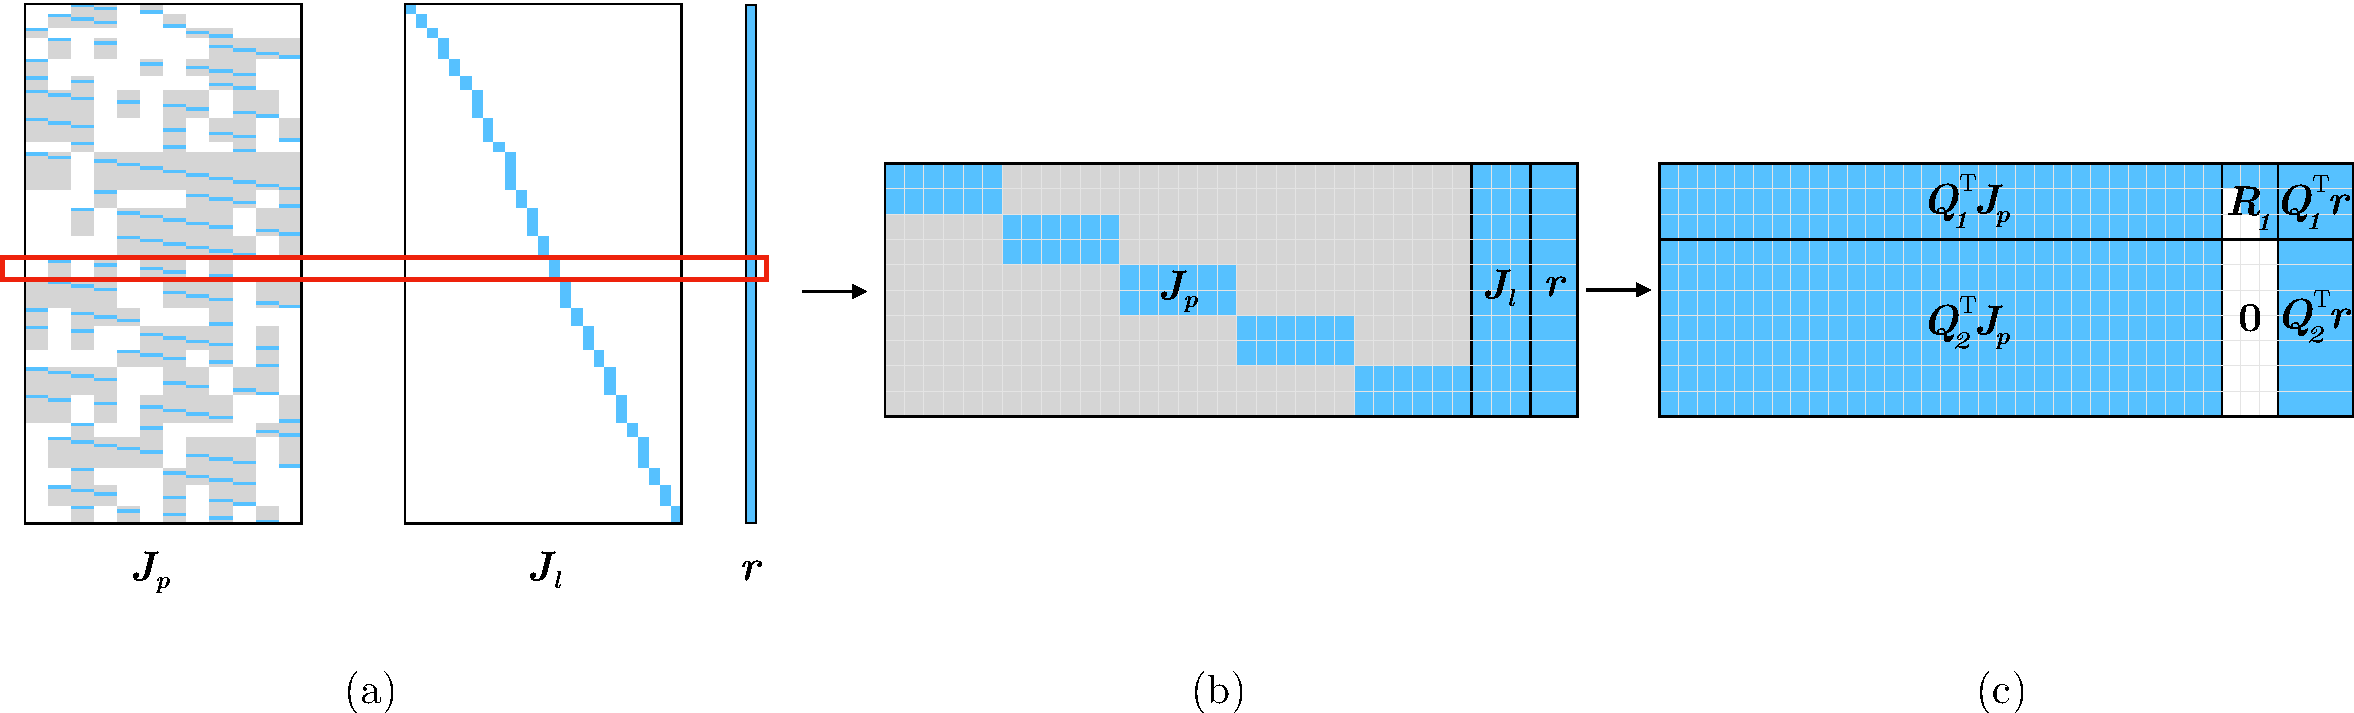
\includegraphics[width=0.9\linewidth]{img/prev_concepts/qr-ba.pdf}
    \caption{Factorización QR.}
    \label{fig:qr-ba}
\end{figure}

\section{Recuperación de imágenes}

\subsection{Modelo Bag of Words}

El modelo de Bag of Words (BoW) es una técnica desarrollada originalmente para la recuperación de texto (\textit{text retrieval}), donde el objetivo es encontrar documentos relevantes en una gran base de datos dada una consulta. La suposición central es que documentos similares tienden a contener las mismas palabras, o al menos una distribución similar de ellas. Un documento puede representarse como un vector en el que cada elemento corresponde a una palabra específica del vocabulario, con su valor codificando si la palabra aparece (representación binaria) o con qué frecuencia lo hace. La similitud entre documentos se mide comparando estos vectores mediante métricas de distancia estándar.

% figura de bow

Sivic y Zisserman transfirieron esta idea a datos visuales en 2003, dando lugar al modelo de \textit{visual bag of words}. Se extraen features locales de las imágenes y se agrupan en palabras visuales (\textit{visual words}) representativas que conforman un vocabulario. Cada imagen se describe entonces por la distribución de esas palabras entre sus features. El agrupamiento o clustering se realiza típicamente mediante k-means o métodos jerárquicos, y dado que los descriptores son de alta dimensionalidad, se necesitan vocabularios de miles a cientos de miles de términos para obtener representaciones suficientemente discriminativas. El retrieval se hace eficiente almacenando las imágenes en un índice invertido indexado por visual word. Dada una imagen de consulta, se calcula su vector BoW y se compara con los almacenados en la base de datos mediante algún método de scoring, como L1, L2, o la similitud del coseno. Las imágenes resultantes se ordenan por similitud y la coincidencia más cercana se devuelve como candidata.

En este trabajo, los features locales utilizados son los descriptores ORB. ORB mejora el detector FAST produciendo features a múltiples escalas con una orientación asociada, que se utiliza para calcular una versión invariante a la rotación y escala del descriptor BRIEF. El resultado es un descriptor binario compacto de 256 bits, eficiente de extraer y comparable mediante la distancia de Hamming.

Las principales ventajas de los modelos BoW son su invarianza implícita al punto de vista, ya que descartan la disposición geométrica de los features, y su eficiencia gracias al índice invertido y las estructuras jerárquicas de vocabulario. Su principal limitación es la susceptibilidad al \textit{perceptual aliasing}, que se muestra en la Figura \ref{fig:perceptual-aliasing}: distintos lugares con apariencia visual similar pueden producir representaciones de bag of words parecidas, lo que lleva a reconocimientos de lugar incorrectos. Este es un desafío fundamental en cualquier sistema de place recognition basado en apariencia.

\begin{figure}[ht]
    \centering
    \begin{subfigure}[b]{0.32\textwidth}
        \centering
        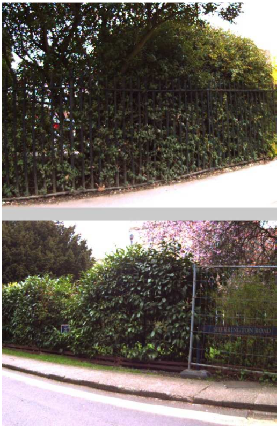
\includegraphics[width=\textwidth]{img/prev_concepts/perceptual-aliasing-1.pdf}
    \end{subfigure}
    \hfill
    \begin{subfigure}[b]{0.32\textwidth}
        \centering
        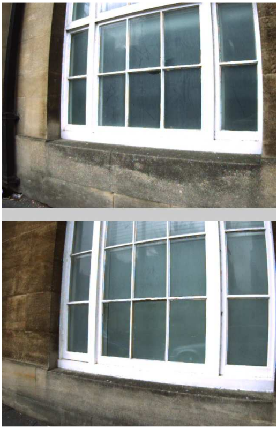
\includegraphics[width=\textwidth]{img/prev_concepts/perceptual-aliasing-2.pdf}
    \end{subfigure}
    \hfill
    \begin{subfigure}[b]{0.32\textwidth}
        \centering
        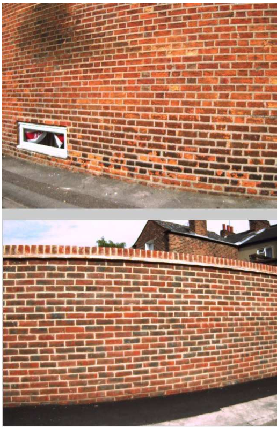
\includegraphics[width=\textwidth]{img/prev_concepts/perceptual-aliasing-3.pdf}
    \end{subfigure}
    % TODO: corregir este caption
    \caption{Imagen extraída de HashBow, que a su vez la extrajo de Cummins and Newman [16, p. 2045].}
    \label{fig:perceptual-aliasing}
\end{figure}

Entre los métodos más destacados que siguen este paradigma se encuentran DBoW, que construye un árbol de vocabulario jerárquico a partir de descriptores binarios mediante clustering con k-medians, y HBST, que organiza los descriptores en un árbol de búsqueda binario indexado por valores de bits para aproximar la búsqueda del vecino más cercano de forma eficiente.

\subsection{HashBoW}

HashBoW es un método de recuperación de imágenes (\textit{image retrieval}) basado en el modelo de bag of words. Discretiza el espacio de descriptores mediante hashing y trata directamente los hashes como palabras visuales, como se puede observar en la Figura \ref{fig:hashbow}.

\begin{figure}[h]
    \centering
    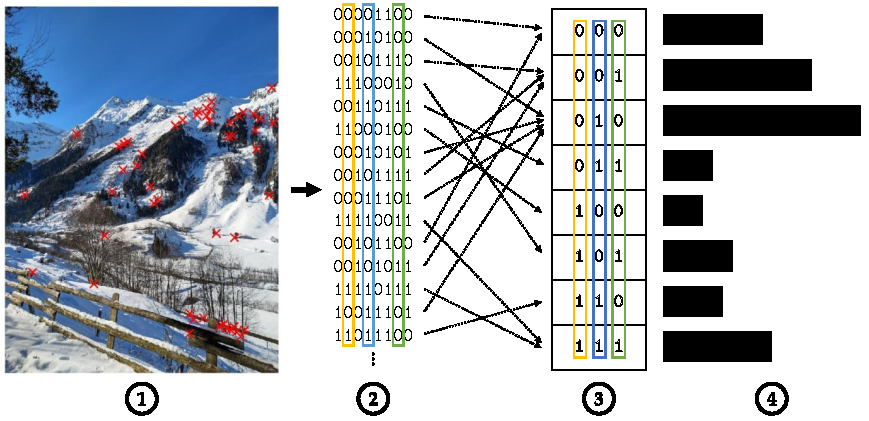
\includegraphics[width=0.8\linewidth]{img/prev_concepts/hashbow.pdf}
    \caption{En el vector de salida, todas las entradas suman 1.}
    \label{fig:hashbow}
\end{figure}

\textit{Locality-sensitive hashing} (LSH) es una estrategia de hashing en la que la función hash está diseñada de modo que elementos similares tengan más probabilidad de ser asignados al mismo bucket que elementos distintos. Esto es especialmente útil para la búsqueda aproximada del vecino más cercano en espacios de alta dimensionalidad. En el contexto de place recognition, LSH proporciona una forma eficiente y teóricamente fundamentada de agrupar descriptores similares.

Aunque puede generalizarse, el método opera exclusivamente sobre descriptores binarios. Una familia LSH simple para descriptores binarios bajo la distancia de Hamming se obtiene mediante \textit{bit sampling}: sea $d$ la dimensión de un descriptor binario $p\in\{0,1\}^d$, cada función hash $h_i(p)=p_i$ simplemente lee el valor en un índice de bit específico $i$. Dicha función cumple con la definición de LSH (el detalle de la definición que demuestra que satisface las propiedades de LSH puede encontrarse en la Definición 2 de la Sección 4.3.3 de -), lo que significa que descriptores cercanos en distancia de Hamming tienen más probabilidad de recibir el mismo valor hash que descriptores lejanos. Para aumentar la expresividad, $n$ de estas funciones se concatenan en un hash combinado $g(p)=(h_1(p),\ldots,h_n(p))$, produciendo un vocabulario de tamaño $N_\text{voc} = 2^n$ donde cada código hash corresponde a una visual word. La longitud del código hash $n$ es, por tanto, el parámetro principal que controla el equilibrio entre expresividad del vocabulario y costo computacional.

Dado que índices de bits elegidos aleatoriamente pueden distribuir los descriptores de forma desigual, HashBoW utiliza un procedimiento de entrenamiento basado en entropía para seleccionarlos. Los índices de bits se eligen de forma greedy y secuencial, seleccionando en cada paso el índice que maximiza la entropía de la distribución hash resultante condicionada a los índices ya seleccionados. Esto garantiza que el vocabulario discretice el espacio de descriptores de la manera más uniforme posible para un conjunto de imágenes de entrenamiento.

Comparado con otros métodos, HashBoW tiene la ventaja de utilizar una transformación de features locales a palabras visuales más simple. Esto tiene como consecuencia una mayor eficiencia, pero también una menor precisión en el retrieval (Véase Figura \ref{fig:hashbow-results}). Esto implica que, dentro
de un sistema SLAM, HashBoW debería ir acompañado de verificaciones de consistencia adicionales, para filtrar falsos candidatos a cierre de ciclo. En conjunto, su simplicidad y eficiencia lo convierten en una opción atractiva para la detección de ciclos en entornos no explorados previamente o con recursos computacionales limitados.

\begin{figure}[ht]
    \centering
    \begin{subfigure}[b]{0.48\textwidth}
        \centering
        \includegraphics[width=\textwidth]{img/method/hashbow\_accuracy.pdf}
        \caption{Basalt}
        \label{fig:hashbow_accuracy}
    \end{subfigure}
    \hfill
    \begin{subfigure}[b]{0.48\textwidth}
        \centering
        \includegraphics[width=\textwidth]{img/method/hashbow\_performance.pdf}
        \caption{BasaltLC}
        \label{fig:hashbow_performance}
    \end{subfigure}
    % TODO: corregir este caption
    \caption{Imagen extraída de [...]. Comparativa de HashBoW contra otros métodos de image retrieval.}
    \label{fig:hashbow-results}
\end{figure}

\section{Estimación de pose en sistemas multi-cámara}

\subsection{El Problema de Pose Absoluta No-Central}

La Figura \ref{fig:noncentral_abs_pose} ilustra la geometría del problema
de pose absoluta no-central (\textit{non-central absolute pose}). En computer vision clásica, el modelo de cámara central asume que
todos los rayos de proyección se originan en un único centro óptico. Al
trabajar con sistemas multi-cámara, sin embargo, esta suposición no se
cumple en general, ya que cada cámara tiene su propio centro óptico
desplazado respecto de las demás. Dichos sistemas se describen
mediante el modelo de cámara generalizada \cite{pless2003}, en el
que las observaciones de distintas cámaras se unifican bajo un sistema de
referencia común denominado \textit{body frame} (también llamado
\textit{viewpoint}). Cada observación de imagen se representa como un
\textit{bearing vector} unitario $\mathbf{f}_i$, que
se origina en el centro de su cámara correspondiente y apunta hacia el
landmark 3D observado, y cada cámara tiene un desplazamiento rígido
conocido $\mathbf{v}_{i0}$ respecto del body frame. Esta abstracción
permite tratar un sistema multi-cámara completo como un único sensor
generalizado, a partir del cual se puede estimar una única pose de forma
conjunta utilizando observaciones de todas las cámaras.

El objetivo es recuperar la rotación $\mathbf{R}$ y la traslación
$\mathbf{t}$ del body frame respecto de un sistema de referencia global
conocido, dado un conjunto de correspondencias entre bearing vectors y
puntos 3D del mundo $\mathbf{p}_i^w$ (correspondencias 3D--2D). Esto es
la generalización del clásico problema Perspective-$n$-Point (P$n$P) a
sistemas multi-cámara, conocido como el problema
Non-Perspective-$n$-Point (NP$n$P). Formalmente, la transformación buscada
satisface
\begin{equation}
    \mathbf{R}\left(n_i \mathbf{f}_i + \mathbf{v}_{i0}\right) + \mathbf{t}
    = \mathbf{p}_i^w,
    \label{eq:npnp}
\end{equation}
donde $n_i > 0$ es la profundidad desconocida del $i$-ésimo punto a lo
largo de su bearing vector.

\begin{figure}[h]
    \centering
    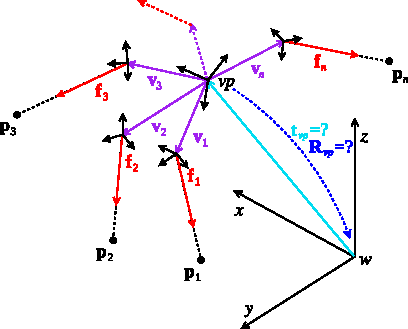
\includegraphics[width=0.55\textwidth]{img/prev_concepts/non-central-abs-pose.pdf}
    \caption{El problema de pose absoluta no-central. Un viewpoint compuesto
             por múltiples cámaras observa un conjunto de puntos 3D del mundo
             mediante bearing vectors $\mathbf{f}_i$. El objetivo es recuperar
             la pose $(\mathbf{R}, \mathbf{t})$ del viewpoint en el sistema de
             referencia global.}
    \label{fig:noncentral_abs_pose}
\end{figure}


\subsection{Los Algoritmos gP3P y gP\textit{n}P}

Kneip et al.\ \cite{kneip2013gpnp} introdujeron dos soluciones eficientes
al problema de pose absoluta no-central. La primera es \textbf{gP3P}, un
solver mínimo que recupera la pose a partir de exactamente tres
correspondencias 3D--2D, potencialmente provenientes de distintas cámaras
del rig, devolviendo hasta ocho soluciones candidatas que se desambiguan
mediante un cuarto punto. La segunda es \textbf{gP$n$P}, un solver de
$n$-puntos no iterativo con complejidad lineal en el número
de correspondencias. Ambos operan directamente sobre bearing vectors y las
transformaciones de cámara a body conocidas, lo que los hace aplicables a
cualquier sistema óptico calibrado. La derivación algebraica completa se
describe en \cite{kneip2013gpnp}.

\subsection{OpenGV}

OpenGV \cite{kneip2014opengv} es una librería de C++ de código abierto que
provee una colección unificada de algoritmos de visión geométrica
calibrada para sistemas de cámara central y no-central, incluyendo gP3P y
gP$n$P. Todos los solvers están integrados dentro de un esquema RANSAC
\cite{fischler1981ransac} y una etapa de refinamiento no lineal bajo una
interfaz común, lo que facilita combinar estimación robusta con recuperación
precisa de pose en un único pipeline.
